\documentclass[pdflatex,compress,mathserif]{beamer}

%\usetheme[dark,framenumber,totalframenumber]{ElektroITK}
\usetheme[darktitle,framenumber,totalframenumber]{ElektroITK}
\usepackage[utf8]{inputenc}
\usepackage[T1]{fontenc}
\usepackage{lmodern}
\usepackage{amsmath}
\usepackage{amsfonts}
\usepackage{amssymb}
\usepackage{graphicx}
\usepackage{multicol}
\usepackage{lipsum}
\setbeamertemplate{caption}[numbered]\setbeamertemplate{caption}[numbered]
\newcommand*{\Scale}[2][4]{\scalebox{#1}{$#2$}}%

\title{Signals and Systems}
\subtitle{The Fourier Transform}

\author{Mifta Nur Farid}

\begin{document}

\maketitle

\begin{frame}
	\frametitle{Discrete Fourier Series to Fourier Transform}
	\begin{figure}
		\centering
		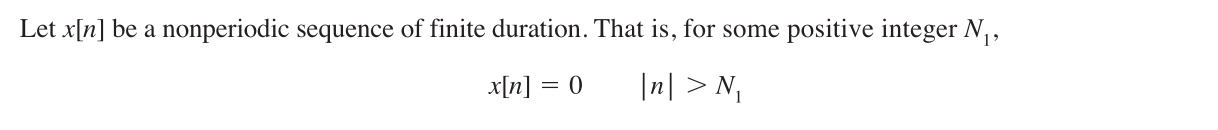
\includegraphics[width=\linewidth]{img/img01}
		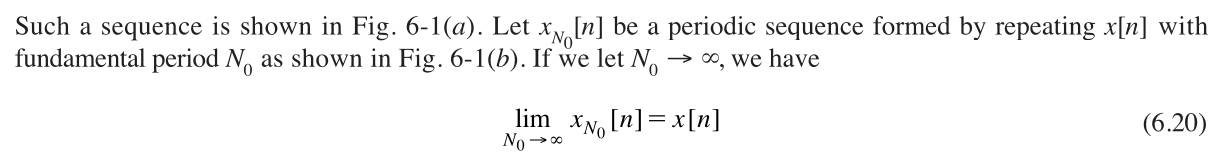
\includegraphics[width=\linewidth]{img/img02}
		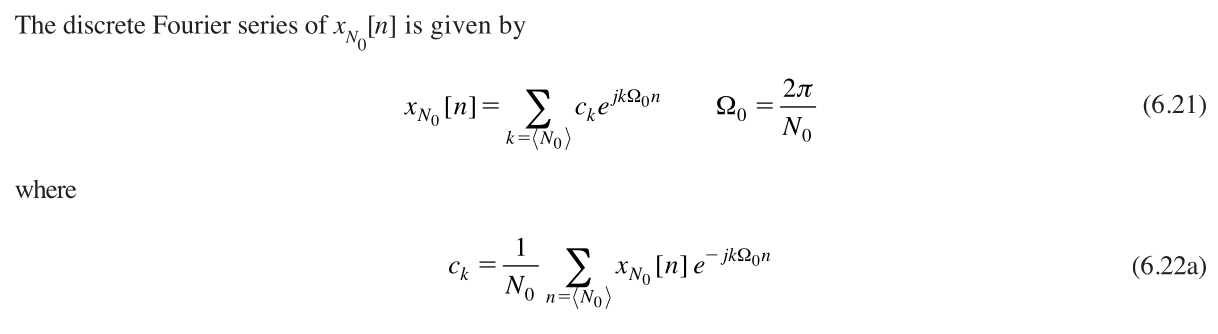
\includegraphics[width=\linewidth]{img/img03}
	\end{figure}
\end{frame}

\begin{frame}{Discrete Fourier Series to Fourier Transform}
	\begin{figure}
		\centering
		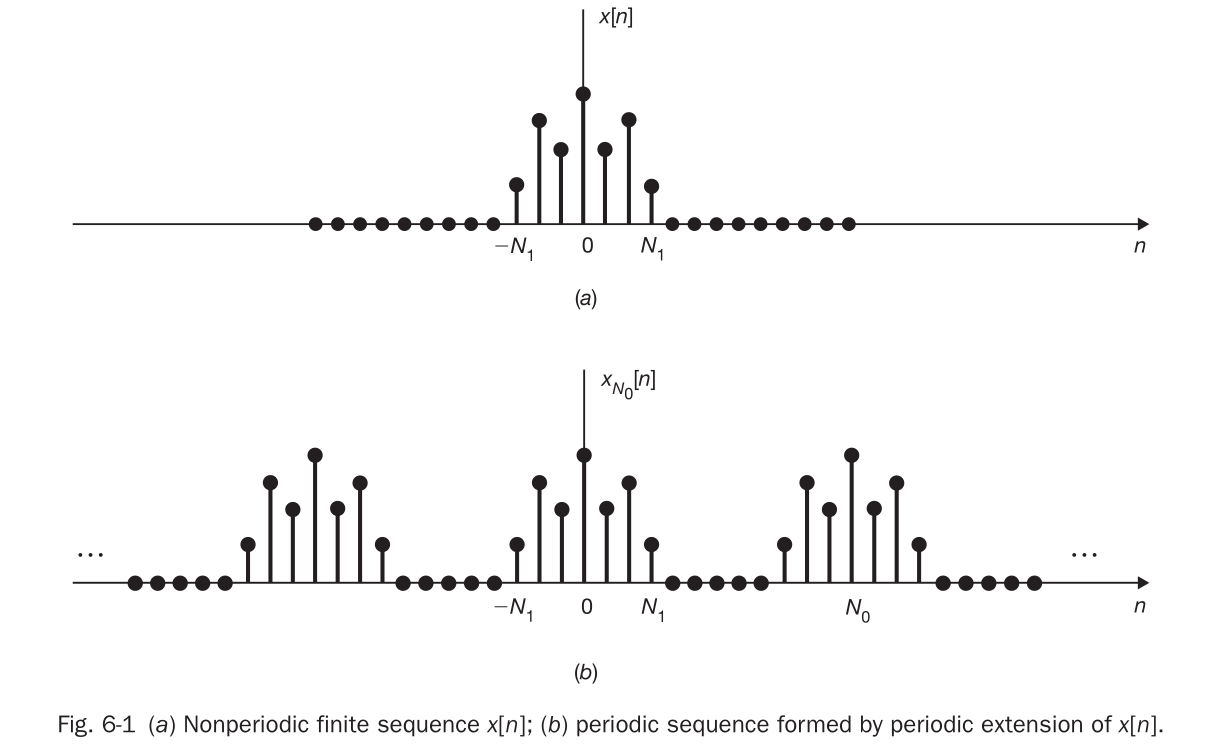
\includegraphics[width=0.9\linewidth]{img/img04}
	\end{figure}
\end{frame}

\begin{frame}{Discrete Fourier Series to Fourier Transform}
	\begin{figure}
		\centering
		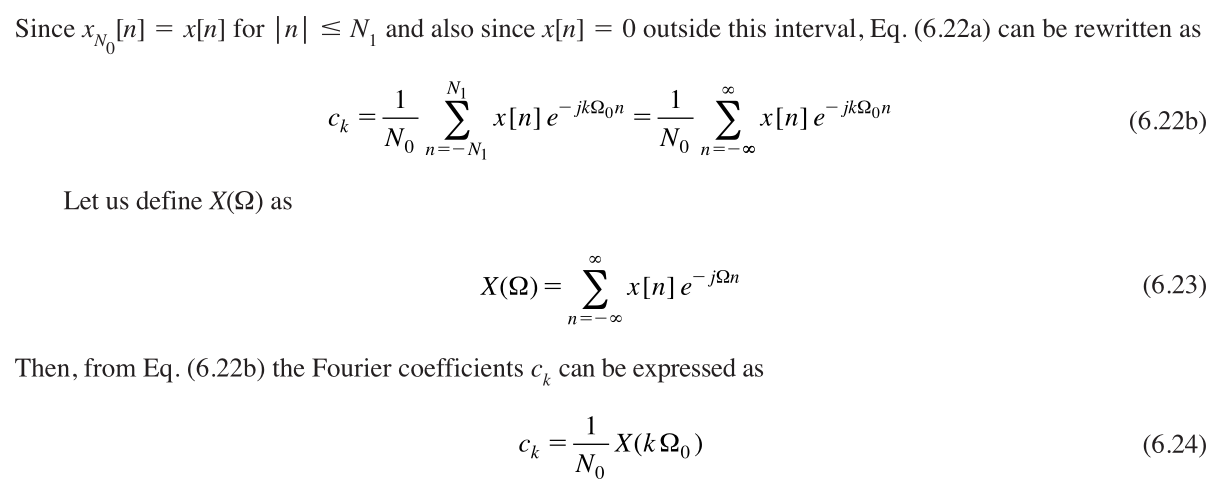
\includegraphics[width=\linewidth]{img/img05}
	\end{figure}
\end{frame}

\begin{frame}{Discrete Fourier Series to Fourier Transform}
	\begin{figure}
		\centering
		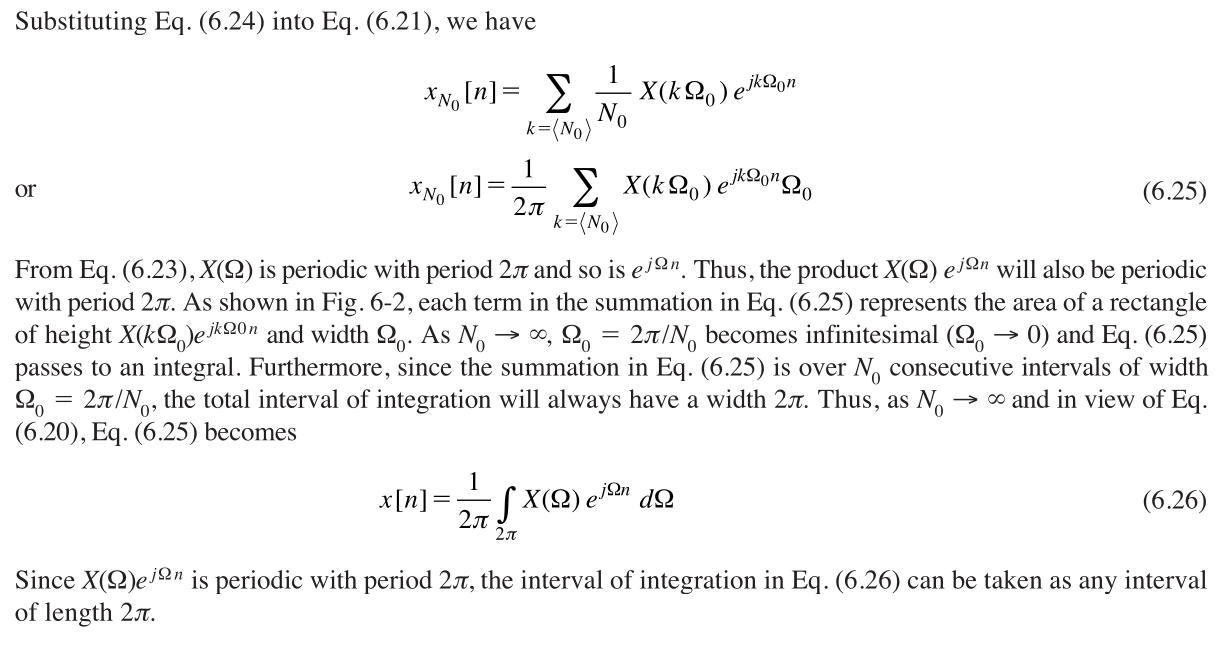
\includegraphics[width=\linewidth]{img/img06}
	\end{figure}
\end{frame}

\begin{frame}{Discrete Fourier Series to Fourier Transform}
	\begin{figure}
		\centering
		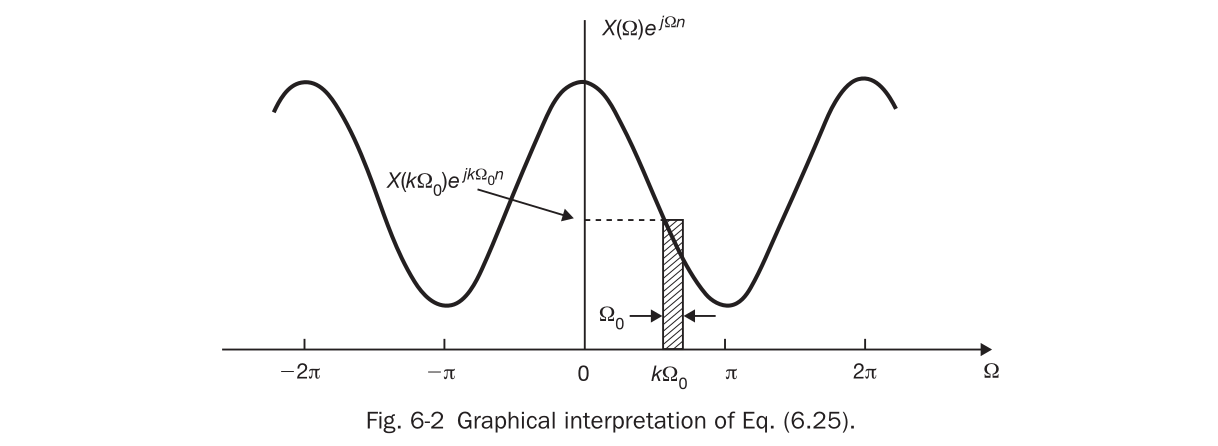
\includegraphics[width=\linewidth]{img/img07}
	\end{figure}
\end{frame}

\begin{frame}
	\frametitle{Fourier Transform Pair}
	\begin{figure}
		\centering
		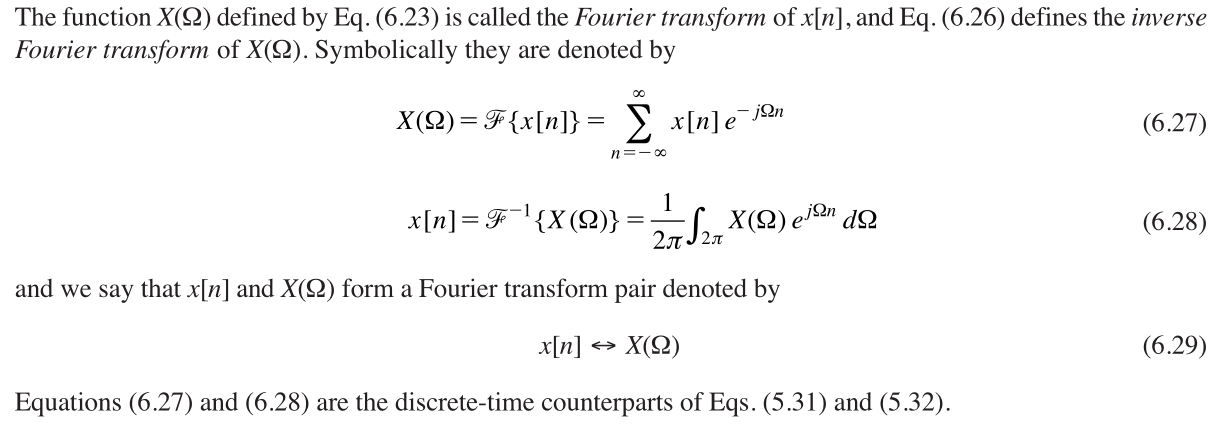
\includegraphics[width=\linewidth]{img/img08}
	\end{figure}
\end{frame}

\begin{frame}
	\frametitle{Fourier Spectra}
	\begin{figure}
		\centering
		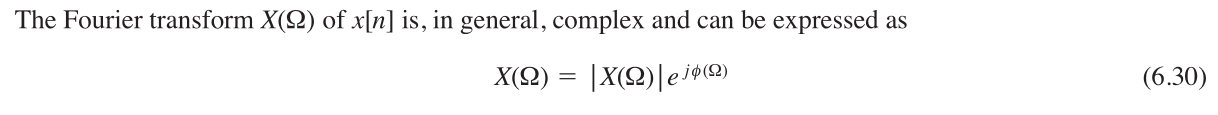
\includegraphics[width=\linewidth]{img/img09}
		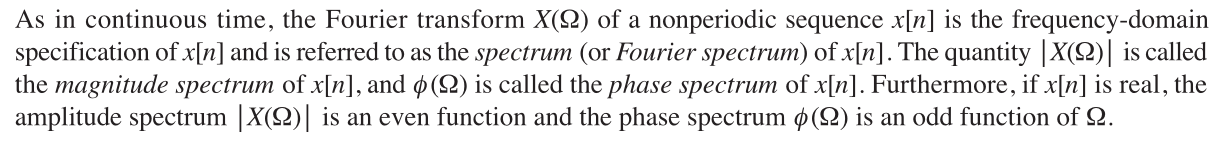
\includegraphics[width=\linewidth]{img/img10}
	\end{figure}
\end{frame}

\begin{frame}
	\frametitle{Convergence of Fourier Spectra}
	\begin{figure}
		\centering
		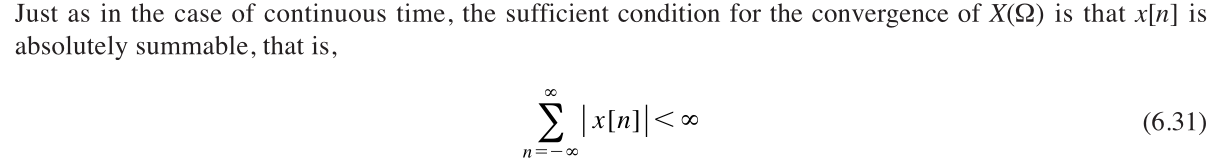
\includegraphics[width=\linewidth]{img/img11}
	\end{figure}
\end{frame}

\begin{frame}
	\frametitle{Properties of the Fourier Transform}
	\begin{figure}
		\centering
		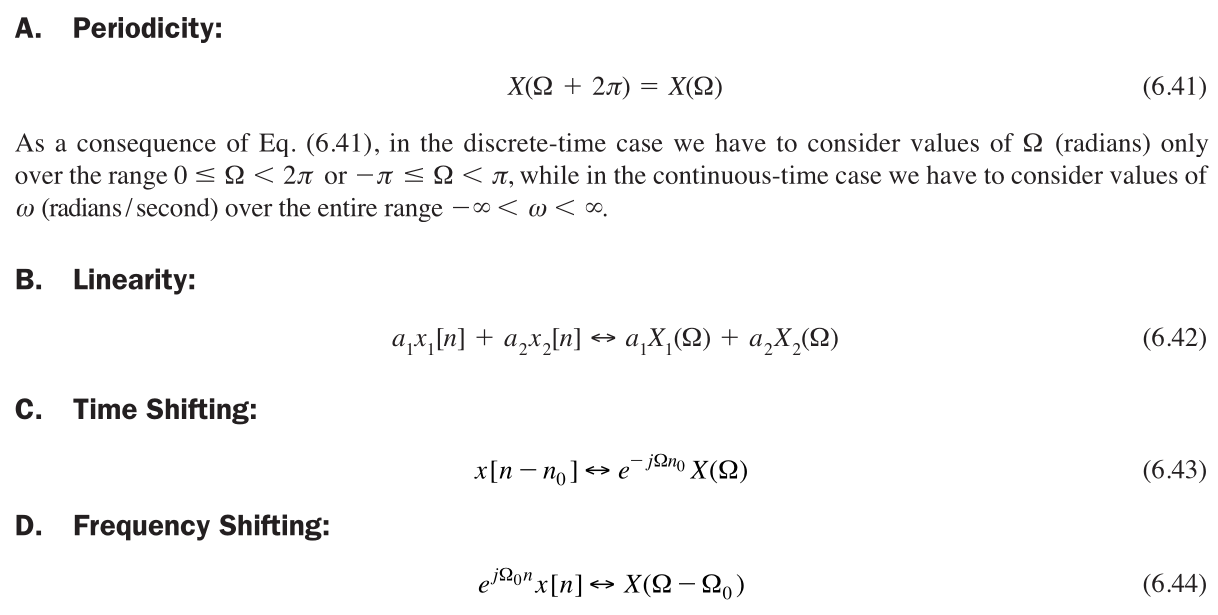
\includegraphics[width=\linewidth]{img/img12}
		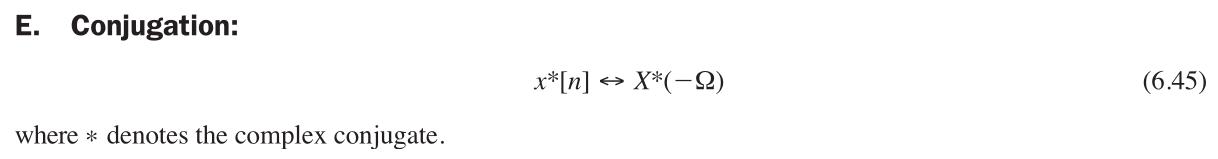
\includegraphics[width=\linewidth]{img/img13}
	\end{figure}
\end{frame}

\begin{frame}{Properties of the Fourier Transform}
	\begin{figure}
		\centering
		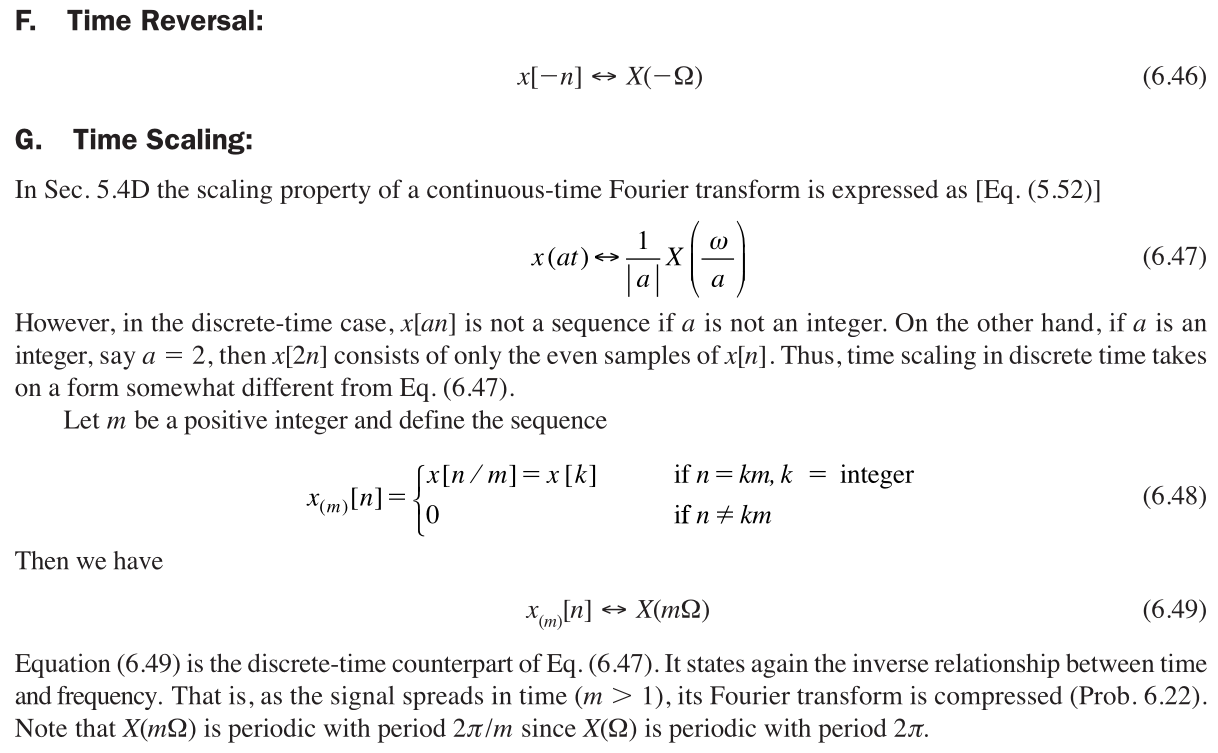
\includegraphics[width=\linewidth]{img/img14}
	\end{figure}
\end{frame}

\begin{frame}{Properties of the Fourier Transform}
	\begin{figure}
		\centering
		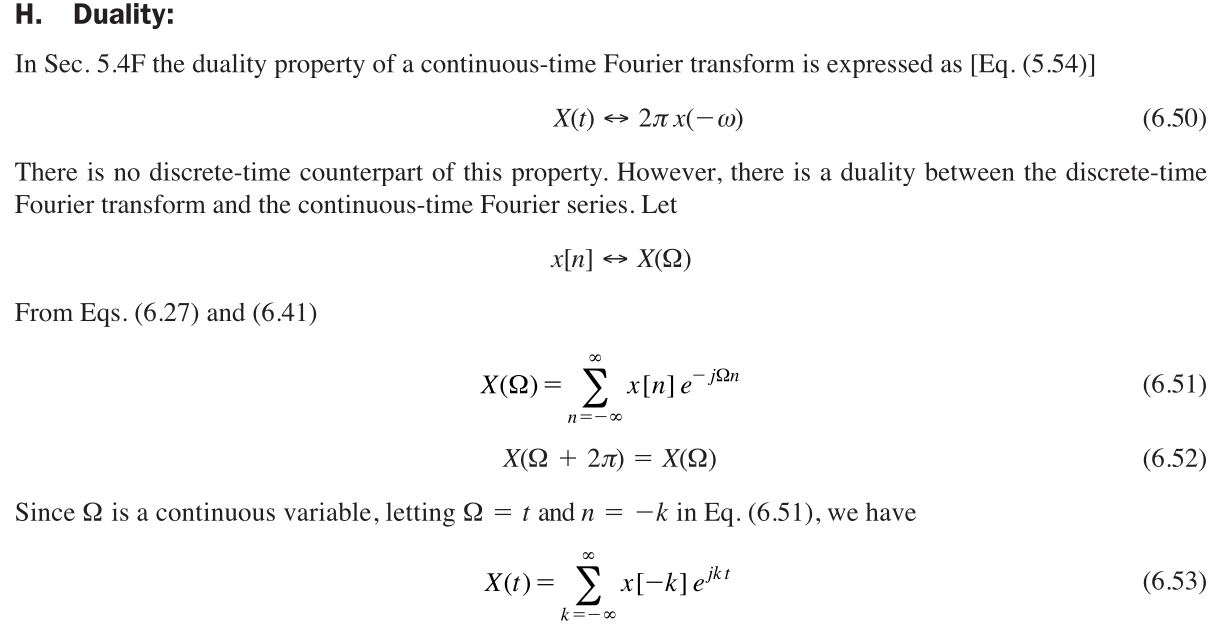
\includegraphics[width=\linewidth]{img/img15}
		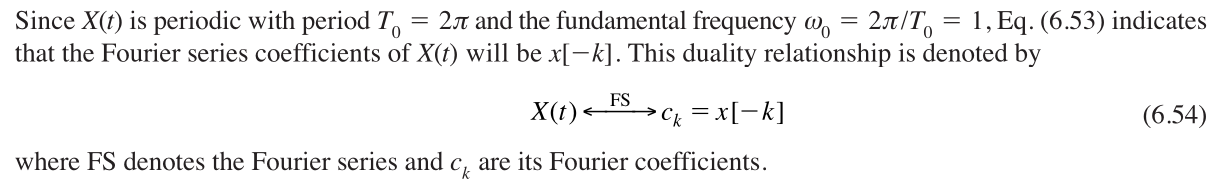
\includegraphics[width=\linewidth]{img/img16}
	\end{figure}
\end{frame}

\begin{frame}{Properties of the Fourier Transform}
	\begin{figure}
		\centering
		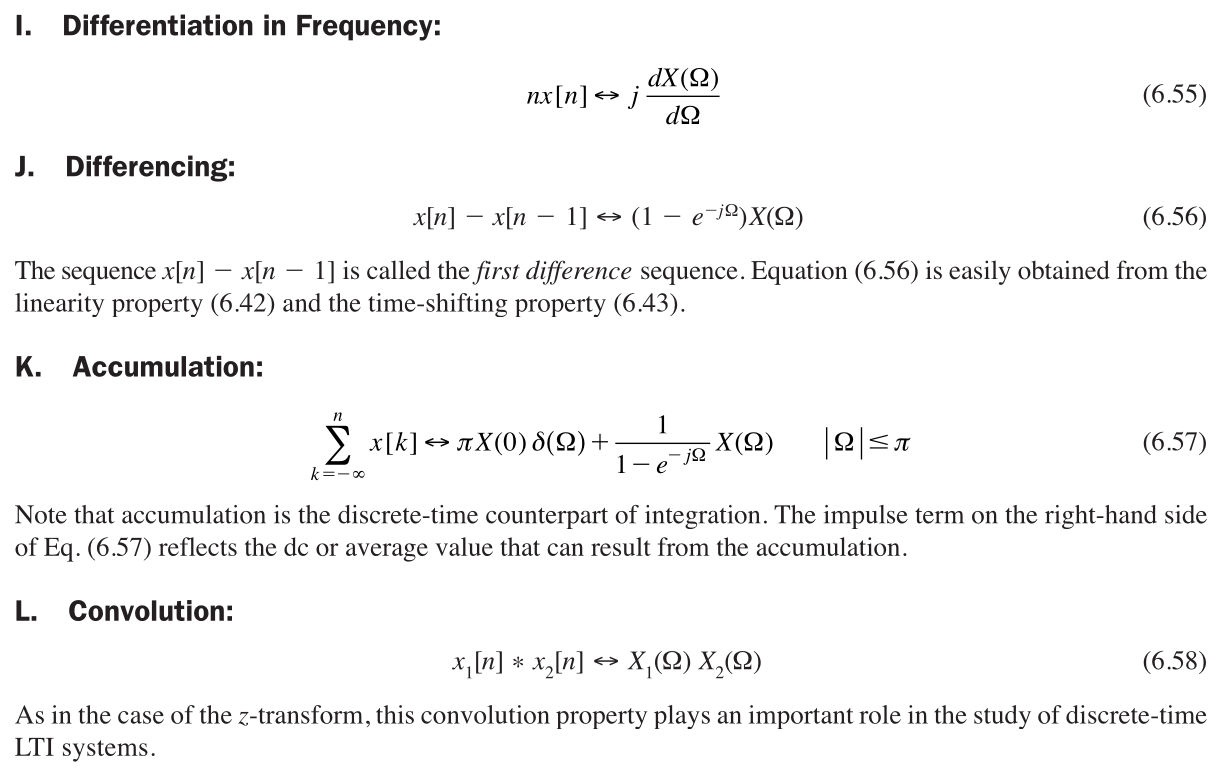
\includegraphics[width=\linewidth]{img/img17}
	\end{figure}
\end{frame}

\begin{frame}{Properties of the Fourier Transform}
	\begin{figure}
		\centering
		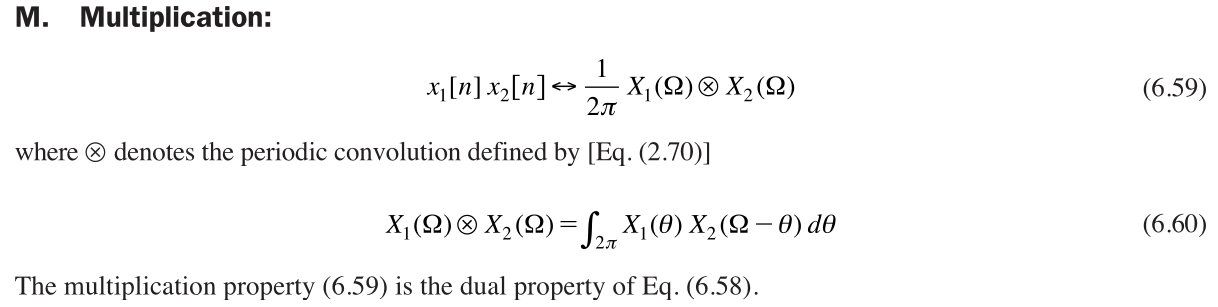
\includegraphics[width=\linewidth]{img/img18}
	\end{figure}
\end{frame}

\begin{frame}{Properties of the Fourier Transform}
	\begin{figure}
		\centering
		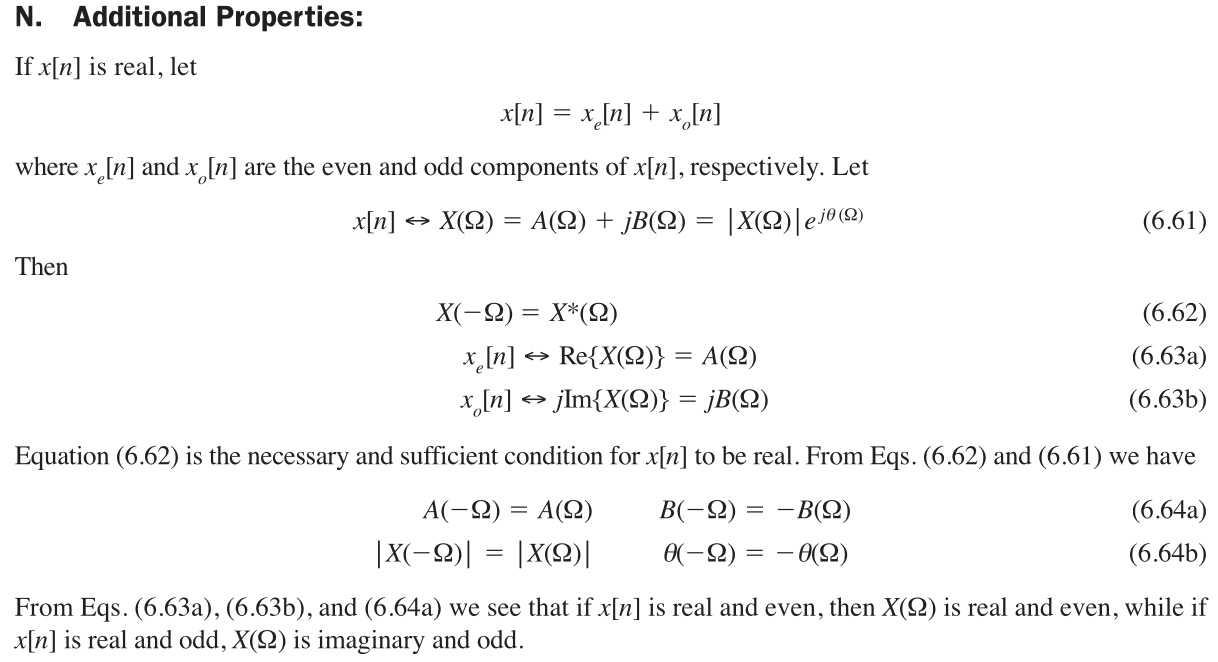
\includegraphics[width=\linewidth]{img/img19}
	\end{figure}
\end{frame}

\begin{frame}{Properties of the Fourier Transform}
	\begin{figure}
		\centering
		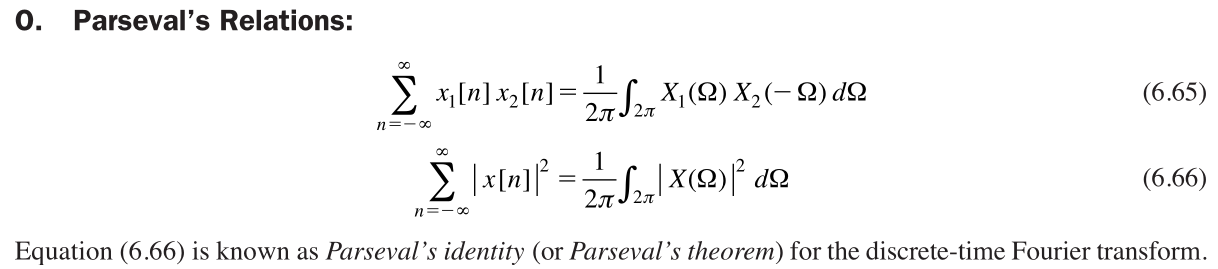
\includegraphics[width=\linewidth]{img/img20}
	\end{figure}
\end{frame}

\begin{frame}
	\frametitle{Common Fourier Transform Pairs}
	\begin{figure}
		\centering
		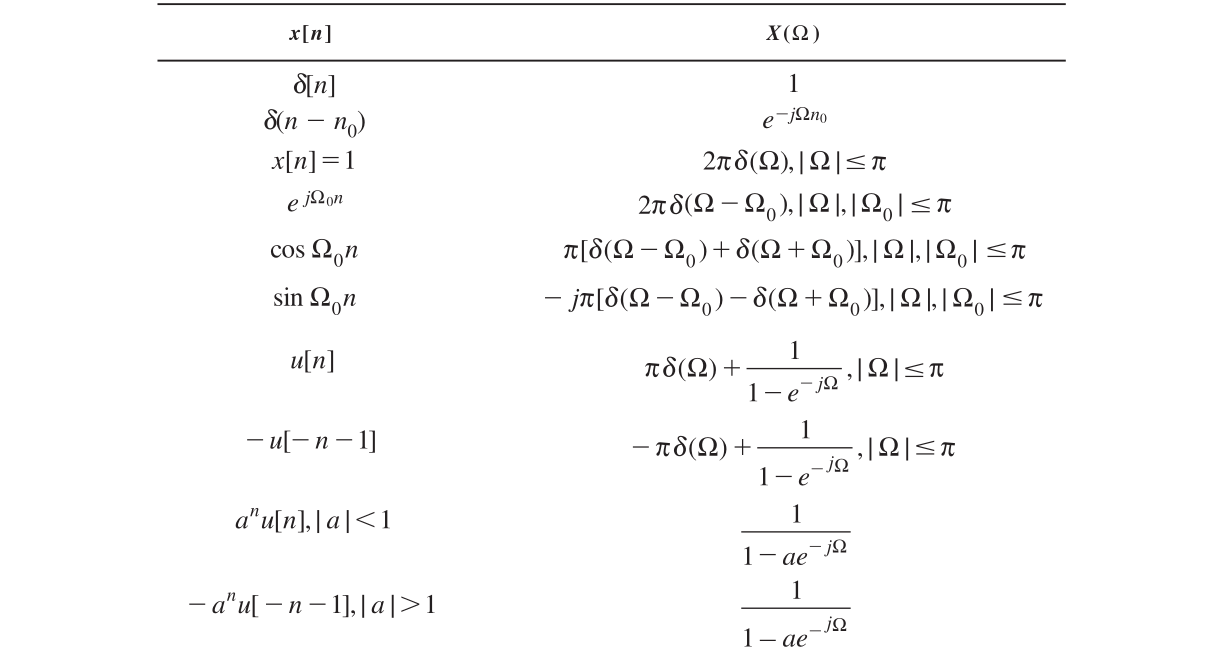
\includegraphics[width=\linewidth]{img/img21}
	\end{figure}
\end{frame}

\begin{frame}{Common Fourier Transform Pairs}
	\begin{figure}
		\centering
		
\includegraphics[width=\linewidth]{img/img22}
		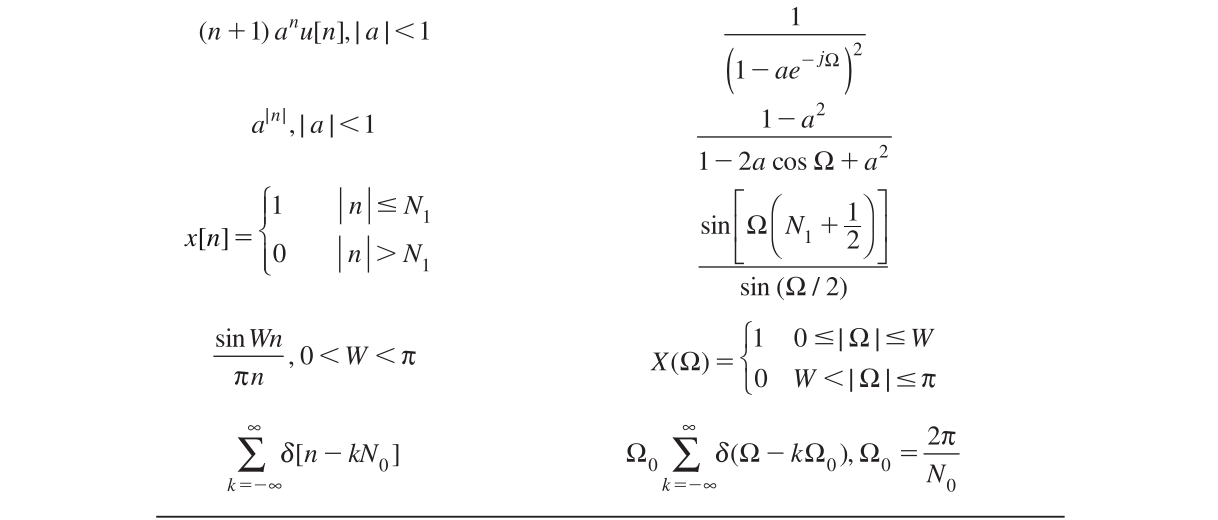
\includegraphics[width=\linewidth]{img/img23}
	\end{figure}
\end{frame}

\begin{frame}
	\frametitle{Latihan Soal}
	\begin{figure}
		\centering
		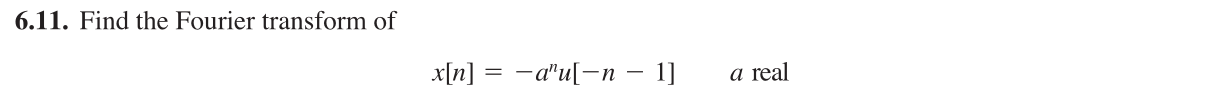
\includegraphics[width=\linewidth]{img/img24}
		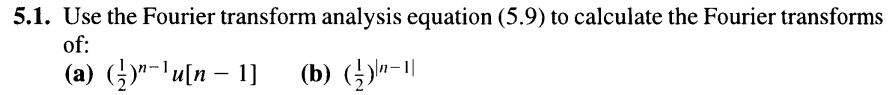
\includegraphics[width=\linewidth]{img/img25}
		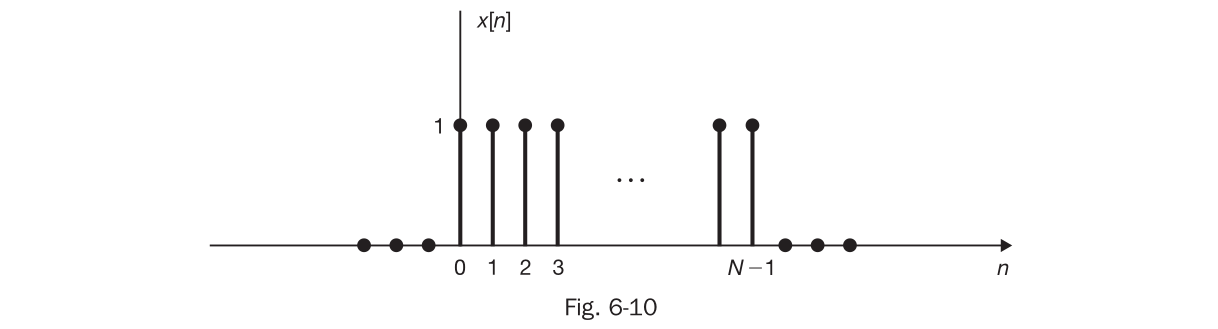
\includegraphics[width=\linewidth]{img/img26}
	\end{figure}
\end{frame}

\end{document}
